\documentclass[10pt]{article}
\usepackage[T1]{fontenc}
\usepackage{lmodern,amsmath,amssymb,booktabs,array,graphicx,tikz,pgfplots}
\usepackage[paperwidth=190mm,paperheight=224mm,margin=10mm]{geometry}
\usepackage[hidelinks]{hyperref}
\hypersetup{pdfauthor={},pdftitle={Monochrome mathematical illustrations: semiconductor-health identifiability}}
\usetikzlibrary{arrows.meta,positioning,calc,patterns}
\pgfplotsset{compat=1.18}
\newcommand{\trans}{^{\mathsf T}}\newcommand{\R}{\mathbb R}
\newcommand{\one}{\mathbf 1}\newcommand{\zero}{\mathbf 0}
\DeclareMathOperator{\rank}{rank}\DeclareMathOperator{\range}{range}
\DeclareMathOperator{\diag}{diag}\DeclareMathOperator{\Cov}{Cov}
\DeclareMathOperator{\Var}{Var}\DeclareMathOperator{\spanop}{span}
\newcommand{\FigureNote}{Visualization code prepared with assistance from OpenAI Codex.}
\pagestyle{empty}\setlength{\parindent}{0pt}
\tikzset{
 every picture/.style={font=\fontsize{9}{11}\selectfont,>=Latex},
 every node/.style={font=\fontsize{9}{11}\selectfont,inner sep=2pt},
 head/.style={font=\fontsize{9.5}{12}\selectfont\bfseries,anchor=west},
 tinytext/.style={font=\fontsize{8}{10}\selectfont},eq/.style={align=center},
 wire/.style={draw=black,line width=.5pt},arr/.style={->,black,line width=.65pt},
 device/.style={draw,fill=white,minimum width=1.1cm,minimum height=.38cm}}
\pgfplotsset{mathaxis/.style={axis lines=left,axis line style={black,line width=.5pt},
 tick style={black},tick label style={font=\fontsize{8}{10}\selectfont},
 label style={font=\fontsize{8.5}{10}\selectfont},grid=major,
 major grid style={black!15,line width=.2pt},
 legend style={font=\fontsize{8}{10}\selectfont,draw=none,fill=white},
 every axis plot/.append style={black}}}
\newcommand{\PlateTitle}[2]{\small\textbf{Mathematical plate #1}\hfill Monochrome TikZ / PGFPlots\par
 \vspace{1.5mm}{\large\bfseries #2}\par\vspace{2mm}}
\newcommand{\PlateCaption}[1]{\par\vspace{1mm}{\fontsize{8.5}{10.5}\selectfont #1\par
 \vspace{1mm}\FigureNote\par}}

\begin{document}
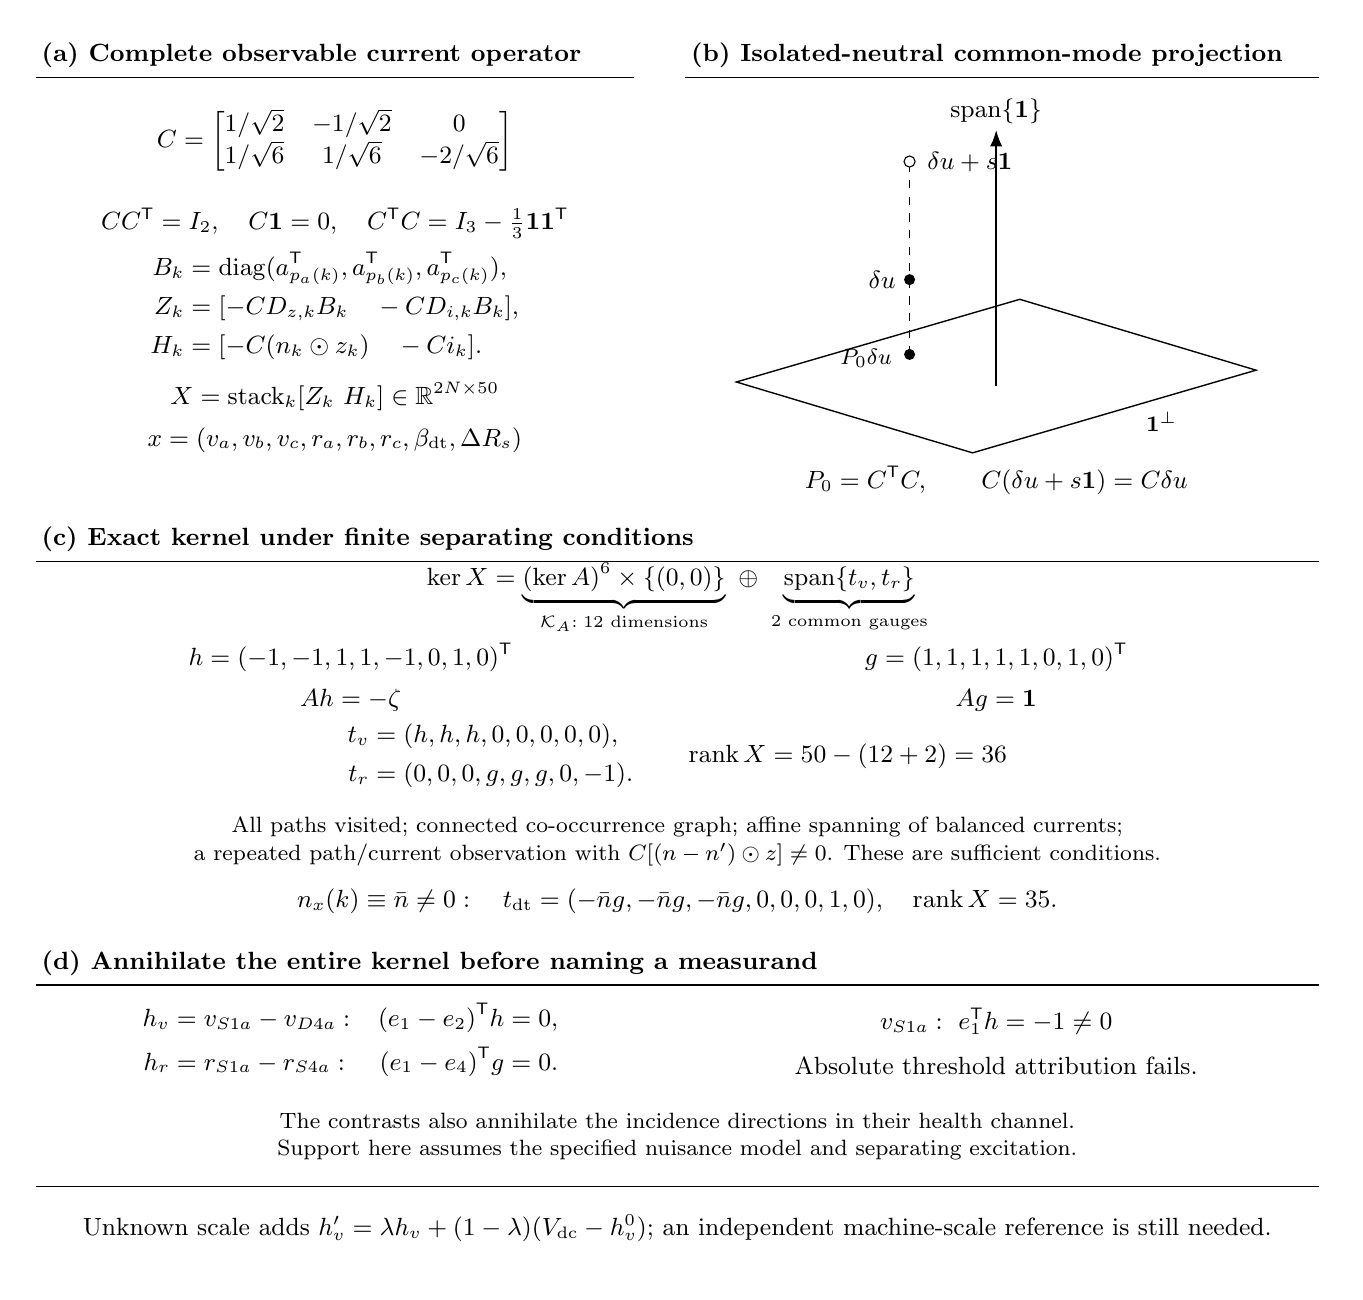
\begin{tikzpicture}[x=1cm,y=1cm]\path[use as bounding box] (0,0) rectangle (16.6,15.8);
\node[head] at (0.1,15.45){(a) Complete observable current operator};\draw[wire] (0.1,15.17)--(7.699999999999999,15.17);
\node[head] at (8.35,15.45){(b) Isolated-neutral common-mode projection};\draw[wire] (8.35,15.17)--(16.4,15.17);
\node[eq] at (3.9,14.36){$C=\begin{bmatrix}1/\sqrt2&-1/\sqrt2&0\\1/\sqrt6&1/\sqrt6&-2/\sqrt6\end{bmatrix}$};
\node[eq] at (3.9,13.32){$CC\trans=I_2,\quad C\one=0,\quad C\trans C=I_3-\tfrac13\one\one\trans$};
\node[eq] at (3.9,12.25){$\begin{aligned}B_k&=\diag(a_{p_a(k)}\trans,a_{p_b(k)}\trans,a_{p_c(k)}\trans),\\
Z_k&=[-CD_{z,k}B_k\quad-CD_{i,k}B_k],\\H_k&=[-C(n_k\odot z_k)\quad-Ci_k].\end{aligned}$};
\node[eq] at (3.9,10.85){$X=\operatorname{stack}_k[Z_k\ H_k]\in\R^{2N\times50}$\\[4pt]
$x=(v_a,v_b,v_c,r_a,r_b,r_c,\beta_{\mathrm{dt}},\Delta R_s)$};
\draw[wire] (9.0,11.3)--(12.0,10.4)--(15.6,11.45)--(12.6,12.35)--cycle;
\node[tinytext] at (14.4,10.8){$\one^\perp$};
\draw[arr] (12.3,11.25)--(12.3,14.5) node[above] {$\spanop\{\one\}$};
\draw[dashed,wire] (11.2,11.65)--(11.2,14.1);
\fill (11.2,12.6) circle(2pt);\node[anchor=east] at (11.1,12.6){$\delta u$};
\draw[fill=white] (11.2,14.1) circle(2pt);\node[anchor=west] at (11.35,14.1){$\delta u+s\one$};
\fill (11.2,11.65) circle(2pt);\node[anchor=east,tinytext] at (11.05,11.6){$P_0\delta u$};
\node[eq] at (12.3,10.05){$P_0=C\trans C,\qquad C(\delta u+s\one)=C\delta u$};
\node[head] at (0.1,9.3){(c) Exact kernel under finite separating conditions};\draw[wire] (0.1,9.020000000000001)--(16.400000000000002,9.020000000000001);
\node[eq] at (8.25,8.55){$\ker X=\underbrace{(\ker A)^6\times\{(0,0)\}}_{\mathcal K_A:\;12\text{ dimensions}}
\ \oplus\ \underbrace{\spanop\{t_v,t_r\}}_{2\text{ common gauges}}$};
\node[eq] at (4.1,7.55){$h=(-1,-1,1,1,-1,0,1,0)\trans$\\[4pt]$Ah=-\zeta$};
\node[eq] at (12.3,7.55){$g=(1,1,1,1,1,0,1,0)\trans$\\[4pt]$Ag=\one$};
\node[eq] at (8.25,6.55){$\begin{aligned}t_v&=(h,h,h,0,0,0,0,0),\\t_r&=(0,0,0,g,g,g,0,-1).
\end{aligned}\qquad\rank X=50-(12+2)=36$};
\node[tinytext,align=center] at (8.25,5.46){All paths visited; connected co-occurrence graph; affine spanning of balanced currents;\\a repeated path/current observation with $C[(n-n')\odot z]\neq0$. These are sufficient conditions.};
\node[eq] at (8.25,4.7){$n_x(k)\equiv\bar n\neq0:\quad t_{\mathrm{dt}}=(-\bar n g,-\bar n g,-\bar n g,0,0,0,1,0),\quad\rank X=35.$};
\node[head] at (0.1,3.92){(d) Annihilate the entire kernel before naming a measurand};\draw[wire] (0.1,3.6399999999999997)--(16.400000000000002,3.6399999999999997);
\node[eq] at (4.1,2.93){$\begin{aligned}
h_v&=v_{S1a}-v_{D4a}:&(e_1-e_2)\trans h&=0,\\
h_r&=r_{S1a}-r_{S4a}:&(e_1-e_4)\trans g&=0.\end{aligned}$};
\node[eq] at (12.3,2.93){$v_{S1a}:\ e_1\trans h=-1\neq0$\\[5pt]Absolute threshold attribution fails.};
\node[tinytext,align=center] at (8.25,1.72){The contrasts also annihilate the incidence directions in their health channel.\\Support here assumes the specified nuisance model and separating excitation.};
\draw[wire] (.1,1.08)--(16.4,1.08);
\node[eq] at (8.25,.55){Unknown scale adds $h_v'=\lambda h_v+(1-\lambda)(V_{\mathrm{dc}}-h_v^0)$; an independent machine-scale reference is still needed.};
\end{tikzpicture}
\end{document}
